% ----------------------------------------------------------------------
%  Pracovní úkoly
% ----------------------------------------------------------------------
\section{Pracovní úkoly}

\begin{enumerate}
\item Změřte charakteristiky Franck-Hertzovy trubice s parami rtuti při teplotách baňky $t_1$=70 °C, $t_2$=110 °C, $t_3$=170 °C. Pro nastavení vhodných parametrů $U_H$, $U_1$, $U_2$ sledujte charakteristiky na osciloskopu.

\item Z naměřených závislostí určete rezonanční potenciál atomů rtuti a vlnovou délku odpovídající rezonančnímu přechodu.

\item Změřte charakteristiku Franck-Hertzovy trubice s neonem až do 99 V. Při měření sledujte, jak se při nárůstu napětí $U_1$ mění počet svítících vrstev v prostoru mezi mřížkami. Pomocí manuálního nastavení napětí $U_1$ určete závislost počtu svítících vrstev na jeho velikosti.

\item Určete rezonanční potenciál atomů neonu a vlnovou délku odpovídající rezonančnímu přechodu.

\end{enumerate}

% ----------------------------------------------------------------------
%  Teoretická část
% ----------------------------------------------------------------------
\section{Teoretická část}

Franckův–Hertzův pokus je experiment, který umožňuje ověřit kvantovou strukturu energie atomů. Jeho princip spočívá ve studiu nepružných srážek elektronů s atomy rtuti (nebo neonu). Elektrony emitované z katody jsou urychlovány napětím $U_1$ směrem k mřížce a dále k anodě (kolektoru). Mezi mřížkou a kolektorem je připojeno malé brzdicí napětí $U_2$, které zajistí, že na kolektor dopadnou pouze elektrony s dostatečně velkou kinetickou energií. Žhavicí napětí $U_H$ řídí emisní proud z katody. 

Při nízkých hodnotách $U_1$ mají elektrony příliš malou energii a s atomy rtuti dochází pouze k pružným srážkám, při nichž elektron téměř neztrácí energii. S rostoucím napětím $U_1$ však může elektron dosáhnout energie odpovídající přechodu z základního do excitovaného stavu atomu. V tomto okamžiku dojde k nepružné srážce a elektron ztratí téměř veškerou svou kinetickou energii. Následkem toho klesá proud na kolektoru, což se projeví jako pokles v charakteristice závislosti proudu na napětí.

Hodnota urychlujícího napětí, při které dochází k prvnímu poklesu, se nazývá \textit{rezonanční potenciál} $U_r$. Odpovídající vlnová délka vyzářeného záření při deexcitaci atomu je dána vztahem
\begin{equation}
    \lambda_r = \frac{hc}{eU_r},
\end{equation}
kde $h$ je Planckova konstanta, $c$ rychlost světla a $e$ elementární náboj.

Při dalším zvýšení napětí může elektron získat dostatečnou energii k ionizaci atomu, čímž dosáhneme \textit{ionizačního potenciálu} $U_i$. Ten je spojen s krátkovlnnou hranicí spektrální série:
\begin{equation}
    \lambda_\infty = \frac{hc}{eU_i}.
\end{equation}

Pro určení $U_r$ se sleduje poloha periodických poklesů v proudově-napěťové charakteristice, které vznikají v důsledku opakovaných nepružných srážek elektronů s atomy. U neonu je navíc rezonanční přechod doprovázen viditelným zářením, takže lze pozorovat vznik svítících vrstev mezi elektrodami.

Chyba je spočtena pomocí metody přenosu chyb \cite{bib:metoda-prenosu-chyb} jako

\begin{equation}
    \sigma = \sqrt{\sum^n_{i=1} \left( \frac{\partial f}{\partial x_i} \right)^2 \sigma^2_{x_i}}
\end{equation}

Odtud nejistota pro vlnovou délku odpovídající rezonančnímu přechodu je spočtena podle

\begin{equation}
    \sigma_{\lambda_r} = \frac{h c}{e U_r^2} \sqrt{\sigma_{U_r}}
\end{equation}

% ----------------------------------------------------------------------
%  Výsledky a zpracování měření
% ----------------------------------------------------------------------
\section{Výsledky a zpracování měření}

\subsection{Páry rtuti}

Nejprve jsme proměřili volt-ampérovou charakteristiku par rtuti při teplotách 70 °C, 110 °C a 170 °C. Tyto závislosti jsou znázorněny na obrázcích \ref{fig:hg-70}, \ref{fig:hg-110} a \ref{fig:hg-170}.

\begin{figure}[!h]
    \centering
    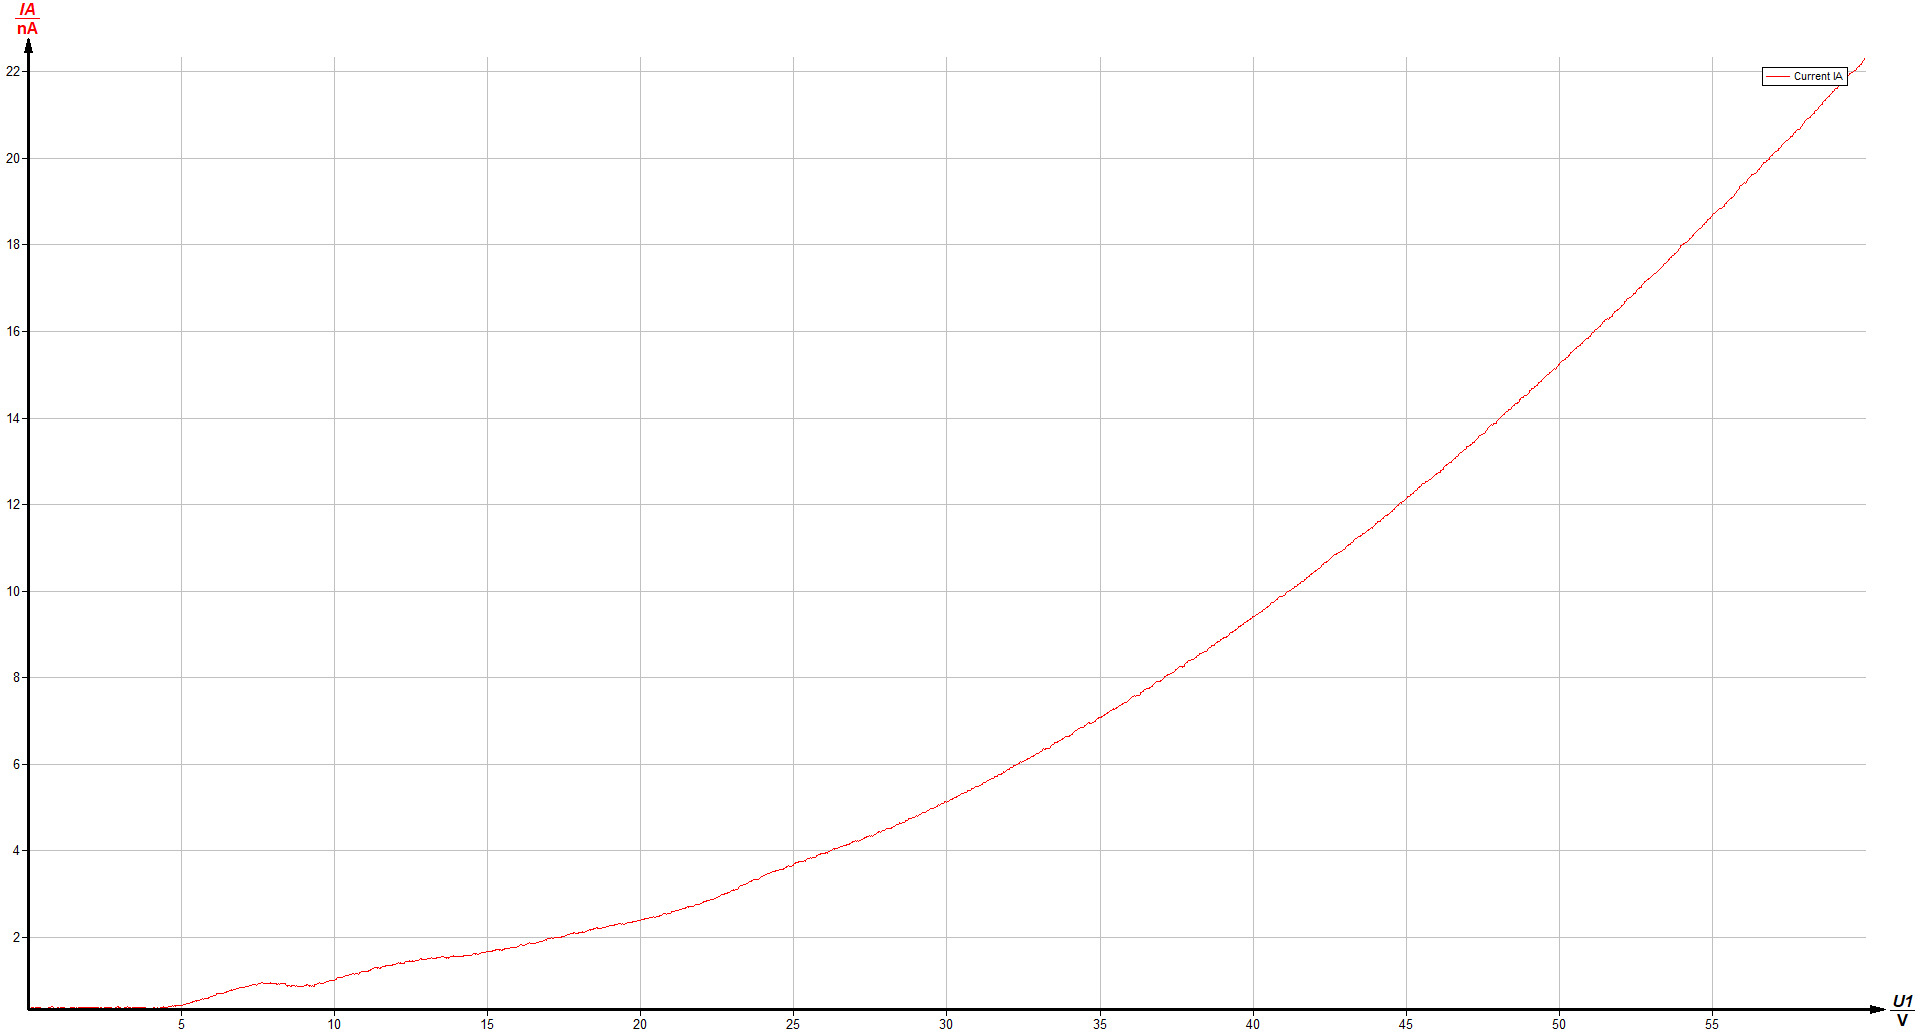
\includegraphics[width=1\linewidth]{A16 - Frank-Hertz/Hg_70.jpg}
    \caption{Charakteristika trubice s parami rtuti při teplotě 70 °C}
    \label{fig:hg-70}
\end{figure}

Pro teplotu 110 °C jsme na grafu vyznačili polohy lokálních maxim.

\begin{figure}[!h]
    \centering
    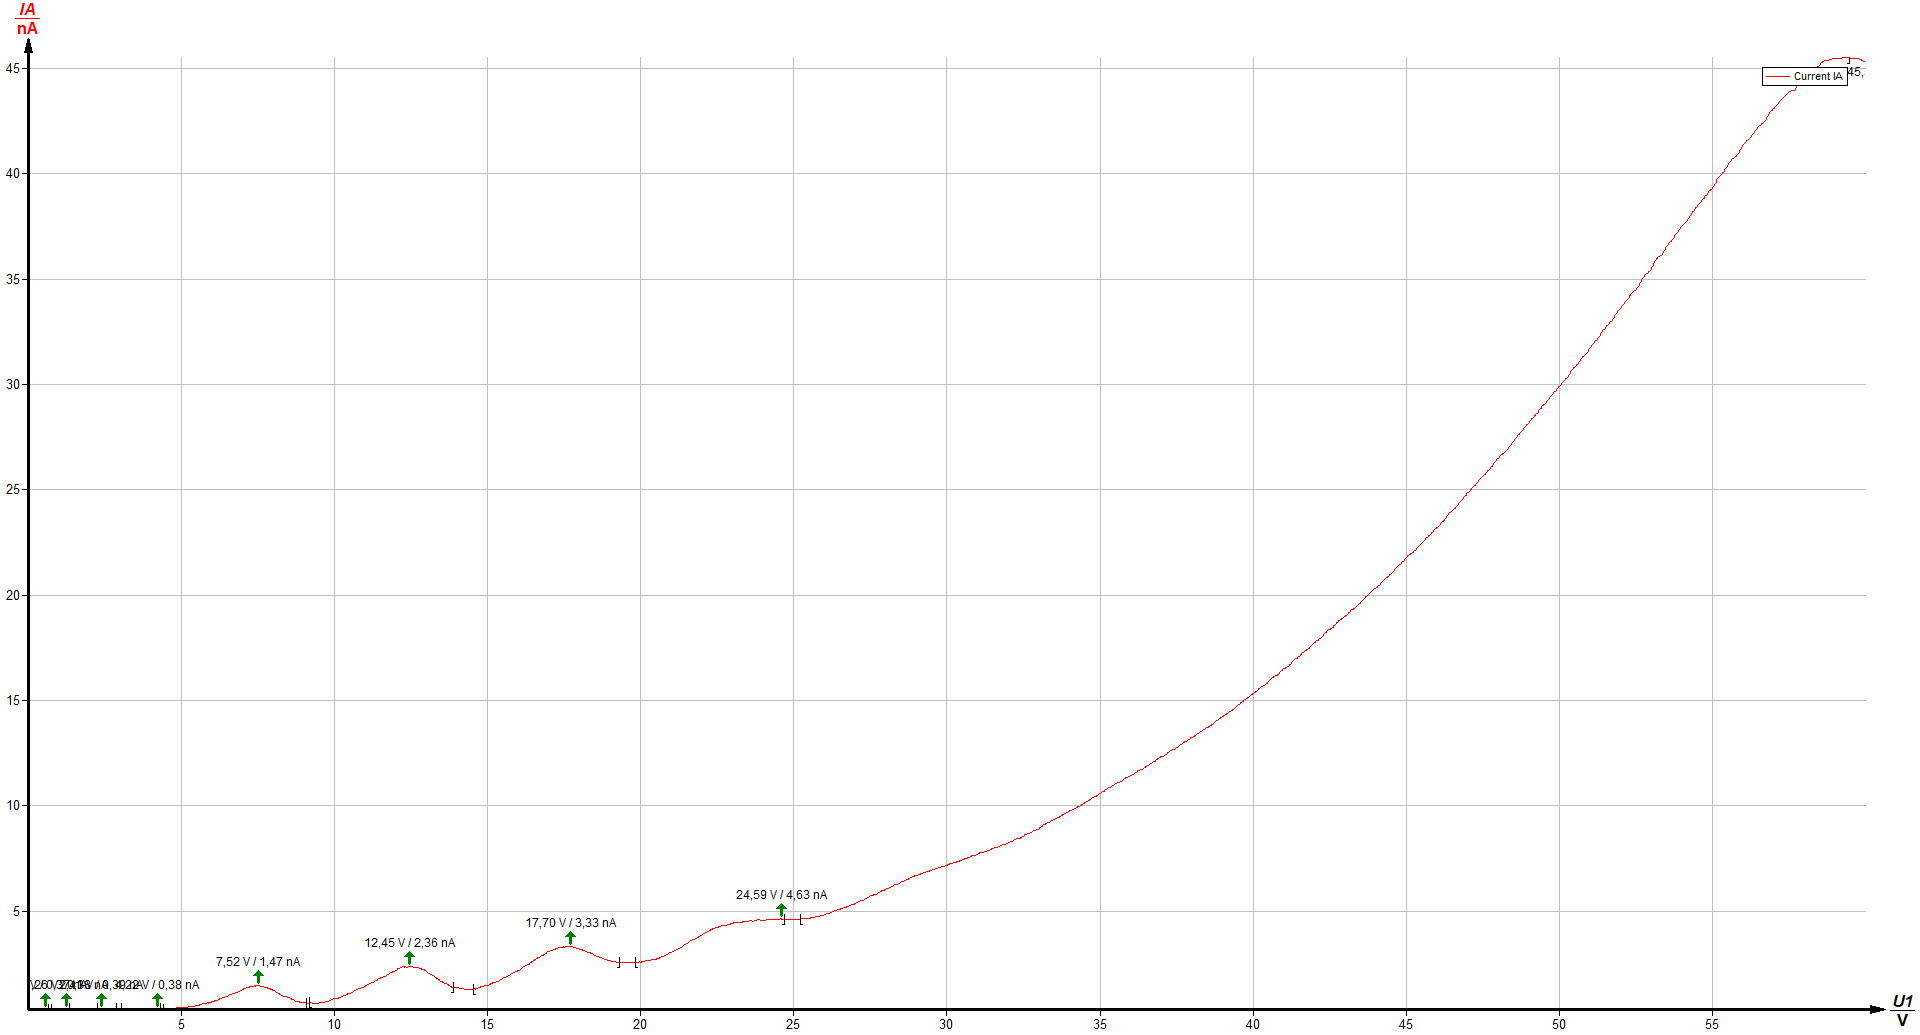
\includegraphics[width=1\linewidth]{A16 - Frank-Hertz/Hg_110.jpg}
    \caption{Charakteristika trubice s parami rtuti při teplotě 110 °C}
    \label{fig:hg-110}
\end{figure}

Pro nejvyšší teplotu 170 °C jsme neměřenou závislost vyhladili (pomocí funkce smooth v programu pro měření) a opět vyznačili lokální maxima.

\begin{figure}[!h]
    \centering
    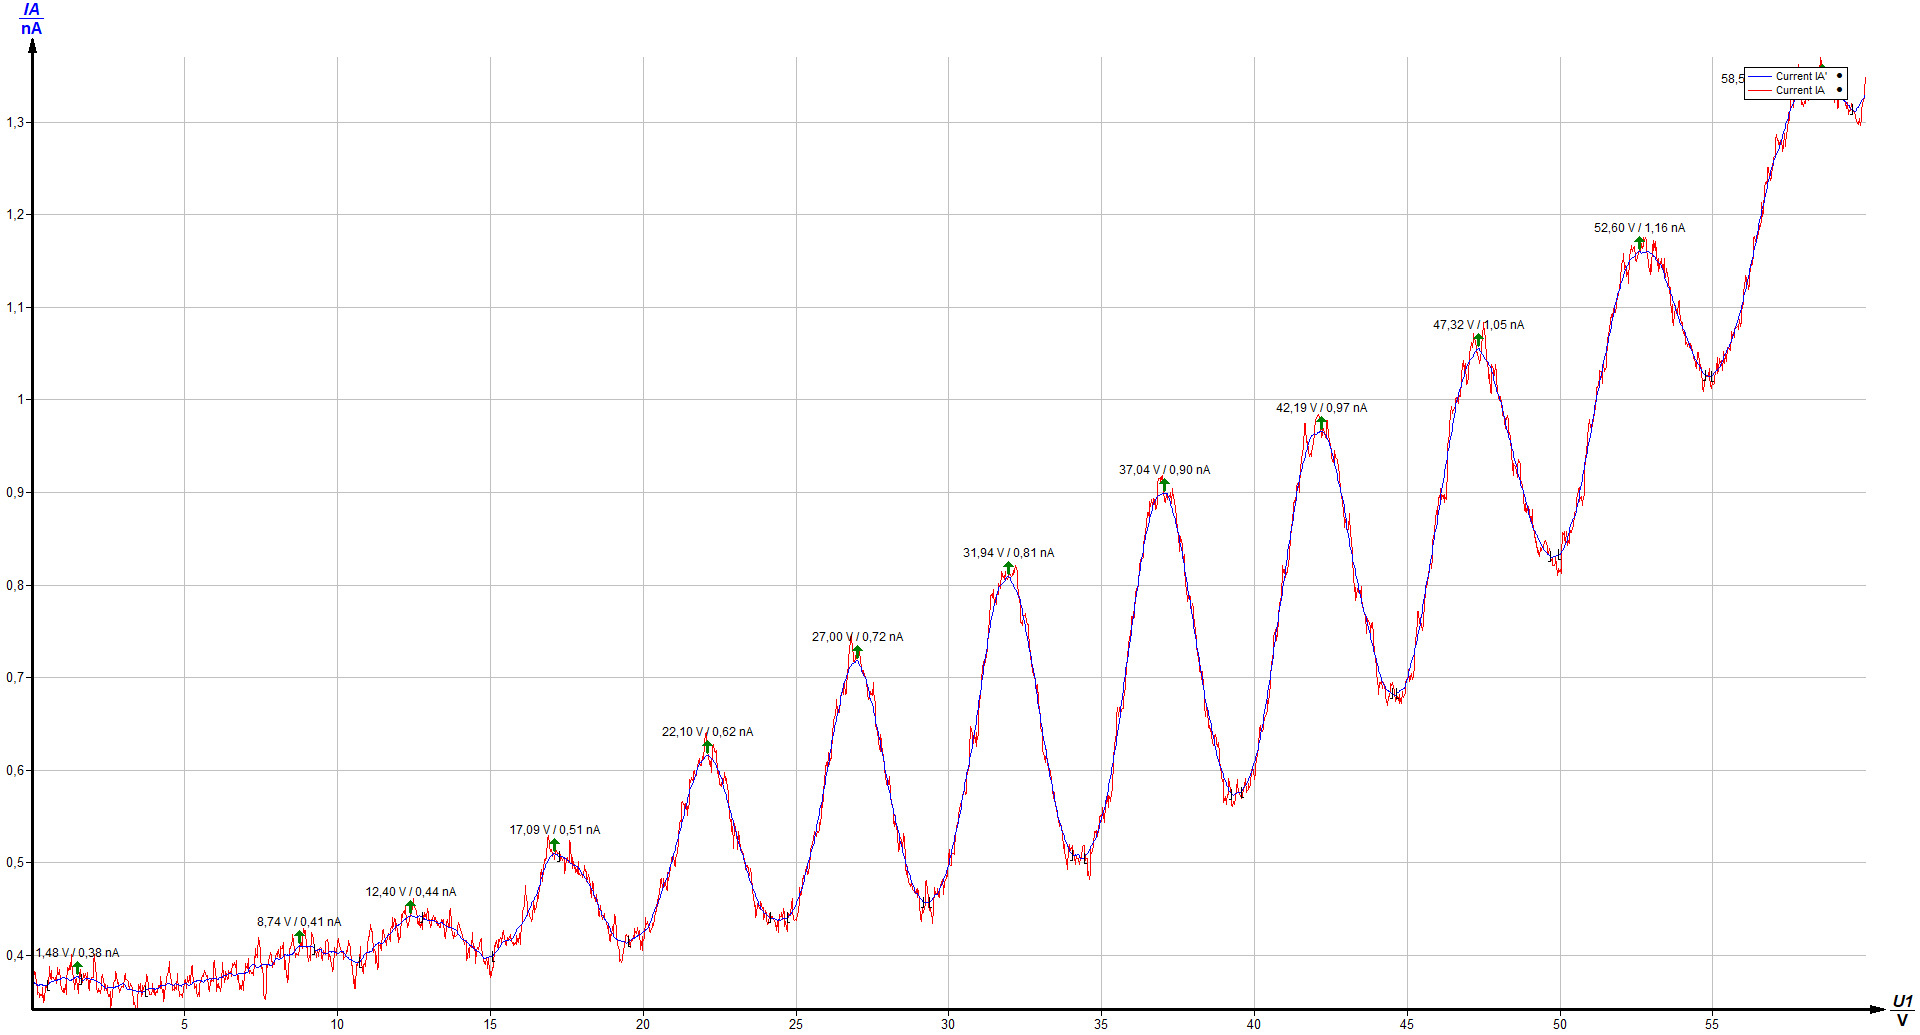
\includegraphics[width=1\linewidth]{A16 - Frank-Hertz/Hg_170.jpg}
    \caption{Charakteristika trubice s parami rtuti při teplotě 170 °C}
    \label{fig:hg-170}
\end{figure}

V tabulce \ref{tab:napeti_FH} jsou zobrazeny parametry jednotlivých měření. Jsou zde uvedeny hodnoty i pro měření neonu, kterému jsme se věnovali v dalším pracovním úkolu.

\begin{table}[!h]
\centering
\caption{Parametry měření pro Ne a Hg při různých teplotách}
\label{tab:napeti_FH}
\begingroup
\setlength{\tabcolsep}{10pt}     % horizontální mezera mezi sloupci
\renewcommand{\arraystretch}{1.2} % vertikální prostrčení řádků
\begin{tabular}{lcccc}
\hline
\textbf{Plyn, teplota} & \textbf{$U_1$ [V]} & \textbf{$U_2$ [V]} & \textbf{$U_3$ [V]} & \textbf{$U_H$ [V]} \\
\hline
Ne & 100 & 7,5 & 5,5 & 5,5 \\
Hg, 110~$^{\circ}$C & 60 & 2,2 & --- & 4 \\
Hg, 70~$^{\circ}$C & 60 & 2 & --- & 3,5 \\
Hg, 170~$^{\circ}$C & 60 & 2 & --- & 5 \\
\hline
\end{tabular}
\endgroup
\end{table}

\newpage

Z těchto naměřených hodnot jsme odečetli rezonanční potenciál jako rozdíl dvou po sobě jdoucích maxim, a to jako

\begin{equation}
    U_{r,Hg} = (5 \pm 0,2) \; V
\end{equation}

kde nejistota je odhadnuta jako průměrná odchylka pro rozdíl různých po sobě jdoucích dvojic maxim. Odtud jsme vypočítali vlnovou délku (s nejistotou podle přenosu chyb podle (4)) odpovídající rezonančnímu přechodu jako

\begin{equation}
    \lambda_{r,Hg} = (247 \pm 22) \; nm
\end{equation}

Tuto vypočtenou hodnotu jsme porovnali s tabulkovou hodnotou

\begin{equation}
    \lambda_{teor,Hg} = 253,7 \; nm
\end{equation}

\newpage

\subsection{Neon}

Podobně jsme proměřili volt-ampérovou charakteristiku neonové trubice. Naměřená závislost s vyznačenými lokálními maximy je zobrazena na obrázku \ref{fig:neon}. Sledovali jsme závislost počtu svítících vrstev v prostoru mezi mřížkami při nárůstu napětí. Tato závislost odpovídá počtu poklesů na grafu, jak předpokládá teorie.

\begin{figure}[!h]
    \centering
    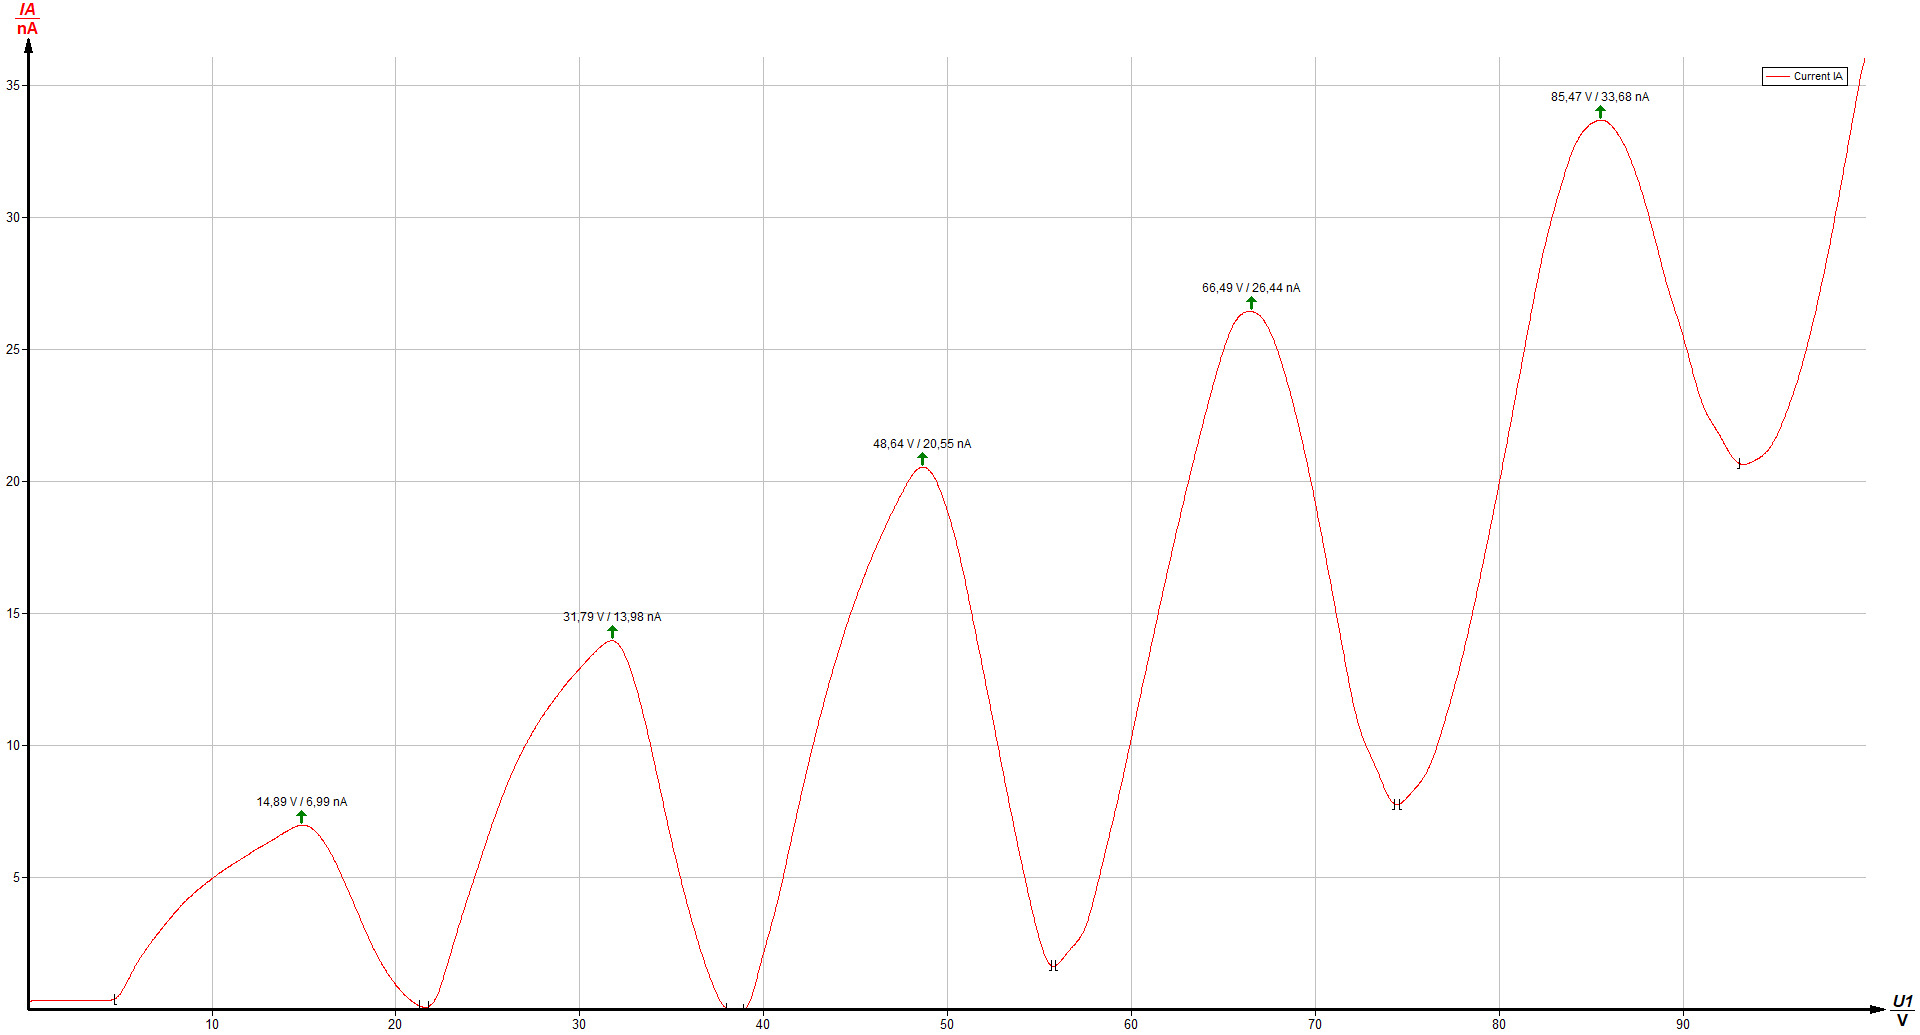
\includegraphics[width=1\linewidth]{A16 - Frank-Hertz/Ne.jpg}
    \caption{Charakteristika trubice s neonem}
    \label{fig:neon}
\end{figure}

Určili jsme rezonanční potenciál na

\begin{equation}
    U_{r,Ne} = (18 \pm 1) \; V
\end{equation}

Odtud spočetli vlnovou délku odpovídající rezonančnímu přechodu

\begin{equation}
    \lambda_{r,Ne} = (68 \pm 50) \; nm
\end{equation}

Tabulková hodnota pro neon je

\begin{equation}
    \lambda_{teor,Ne} = 632,8 \; nm
\end{equation}

Vysoká odlišnost těchto hodnot je rozebrána v sekci diskuse.

    
% ----------------------------------------------------------------------
%  Diskuse výsledků
% ----------------------------------------------------------------------			
\newpage
\section{Diskuse výsledků}

Pro vhodné měření par rtuti bylo nejprve třeba nastavit správné parametry napětí jednotlivých částí obvodu. Při špatném nastavení docházelo například k přesaturování měřeného napětí (hodnoty byly mimo náš rozsah) nebo naopak k příliš nízkým hodnotám napětí a nedostatečnému tak rozlišení. Bylo proto třeba nastavit vhodný vzájemný kompromis mezi těmito parametry. Navíc toto nastavení ovlivňovalo rozpálení pece. To znamená, že v různých časech (například chladnutí pece) byly vhodné jiné parametry.

Hodnotu rezonančního potenciálu jsme odhadli jako průměrnou hodnotu mezi různými po sobě jdoucími maximy. Odlišnost v těchto výsledcích jsme zahrnuli do nejistoty měření.

Jak předpovídala teorie, pro rtuť při teplotě 70 °C závislost odpovídala klasické volt-ampérové charakteristice diody bez výrazných maxim. Při zvyšování teploty dochází k nárůstu počtu poklesů. Při teplotě 170 °C již pozorujeme pouze závislost poklesů.

Porovnáním dopočtené vlnové délky světla pro páry rtuti s tabulkovou hodnotou vidíme, že se měření velmi dobře shoduje. Nejistota je přibližně 4-krát vyšší než rozdíl mezi těmito hodnotami. Naopak pro neon se výsledek řádově neshoduje s tabulkovou hodnotou při zachování stejného postupu výpočtu. Důvodem je složitější spektrum neonu. Naměřená vlnová délka vyzářeného světla neodpovídá celkové deexcitaci atomu na základní stav. Vyzařování probíhá přes mezistupně, proto dostáváme nižší vlnové délky.

Při průběhu měření neonu jsme v trubici pozorovali nárůst počtu svítících vrstev při zvyšujícím se napětí $U_1$. U rtuti jsme tyto vrstvy nepozorovali, protože se nacházejí mimo oblast viditelného světla.

% ----------------------------------------------------------------------
%  Závěr
% ----------------------------------------------------------------------
\section{Závěr}

Franckův–Hertzův pokus poskytuje experimentální důkaz kvantované struktury energetických hladin atomů. Z naměřených dat byl určen rezonanční potenciál rtuti
\[
U_{r,\mathrm{Hg}} = (5 \pm 0{,}2)\,\mathrm{V},
\]
který odpovídá vlnové délce
\[
\lambda_{r,\mathrm{Hg}} = (247 \pm 22)\,\mathrm{nm}.
\]
Naměřená hodnota je v dobré shodě s tabulkovou hodnotou $\lambda_{\mathrm{teor}} = 253{,}7\,\mathrm{nm}$.

U neonu byl rezonanční potenciál
\[
U_{r,\mathrm{Ne}} = (18 \pm 1)\,\mathrm{V},
\]
z čehož vyplývá
\[
\lambda_{r,\mathrm{Ne}} = (68 \pm 50)\,\mathrm{nm}.
\]
Odchylka od tabulkové hodnoty $\lambda_{\mathrm{teor}} = 632{,}8\,\mathrm{nm}$ je způsobena složitějším spektrem neonu a přítomností mezistavů.

Experiment tak potvrdil kvantový charakter energie atomů a umožnil určit rezonanční potenciály rtuti a neonu s odpovídajícími vlnovými délkami.